\documentclass[onecolumn]{article}
\usepackage{graphicx}

\begin{document}
\title{Experiments with catenating arrays in Fortran}
\maketitle

\section{Overview of the experiments}

The basic experiment with the catenation operation involves:
\begin{itemize}
\item
Repeatedly catenate an array of given size.
\item
Access elements of the catenation results, either via a fixed step or randomly (spread over
the entire range)
\item
Measure the time for various step sizes and array sizes
\item
Compare the time with that required for an ordinary array of the same total size.
\end{itemize}

\begin{table}
\caption{Versions of the source files}
\begin{tabular}{ll}
\hline
\verb+view_general.f90+          & Define an object that can hold arrays of any dimension                  \\
                                 & -- basic version                                                        \\
\verb+view_general_v3.f90+       & Use a derived type, not a class                                         \\
\verb+view_general_v4.f90+       & Move determination of the index into the \verb+element_of+ routine      \\
                                 & (use a class again)                                                     \\
\verb+view_general_v5.f90+       & As version 4, but with a derived type                                   \\
\verb+view_general_v6.f90+       & Drop the checks on ranges/indices, use a component \verb+dim+           \\
                                 & instead of a \verb+SIZE()+                                              \\
                                                                                                                                                                                                                                                                                                                                                                                                                                                                                                                                                                                                                                                                                                                                                                                                                                                                                                                                                                                                                                                          \hline
\verb+moa_view_ndim.f90+         & Define an object that can hold the result of a catenation               \\
                                 & -- recursive data structure                                             \\
\verb+moa_view_ndim_alt.f90+     & Use allocatables instead of pointers                                    \\
\verb+moa_view_ndim_flat.f90+    & Alternative implementation: flat array of \verb+moa_basic_view+ objects \\
\verb+moa_view_ndim_flat_v2.f90+ & Optimised version: avoid copying the shape array (just use the          \\
                                 & first element)                                                          \\
\verb+moa_view_ndim_flat_v3.f90+ & Use a derived type instead of a class for \verb+moa_basic_view+         \\
\verb+moa_view_ndim_flat_v4.f90+ & Store the first dimension of \verb+moa_basic_view+ objects in the       \\
                                 & \verb+moa_view_type+, avoiding a function call                          \\
\verb+moa_view_ndim_flat_v5.f90+ & Drop the run-time checks                                                \\


\end{tabular}
\end{table}

section{Implementations}
The first implementation was according to the theory: recursive data types. This implementation was
rather complicated.

The second implementation uses a "flat" data structure. The individual n-dimensional arrays are stored in an
array of type \verb+moa_basic_type+. This makes the implementation much simpler.

Here are a series of plots showing the times we got at various platforms -- "Plain Windows" indicates a laptop,
"Virtual Windows" indicates a virtual machine running Windows and "Linux" indicates a Linux workstation.

\begin{figure}
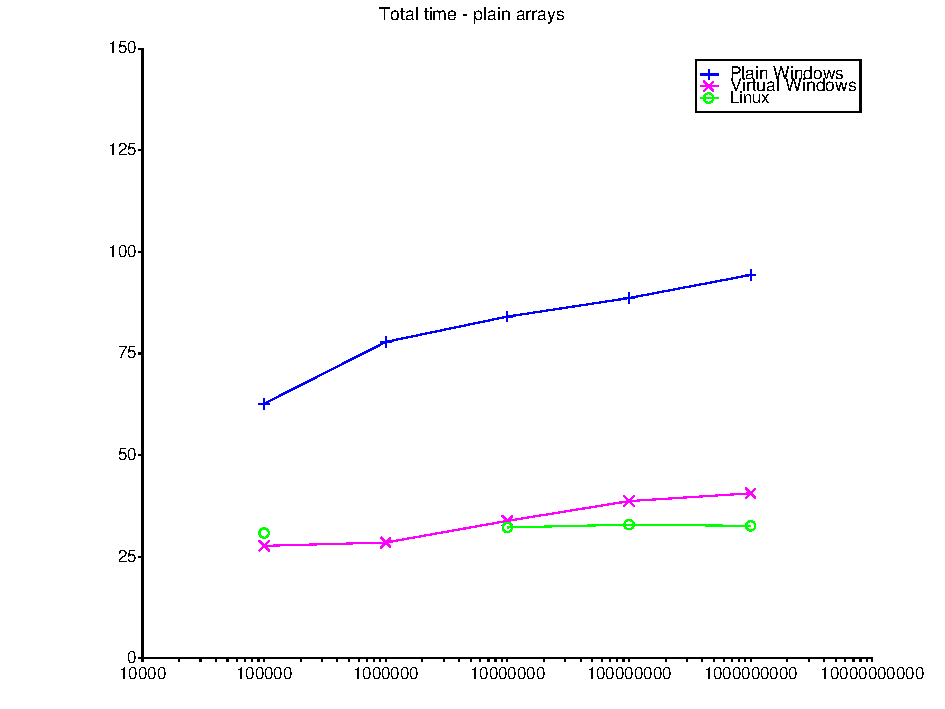
\includegraphics[width=0.9\textwidth]{total_array.pdf}
\caption{Timings using plain arrays}
\end{figure}

\begin{figure}
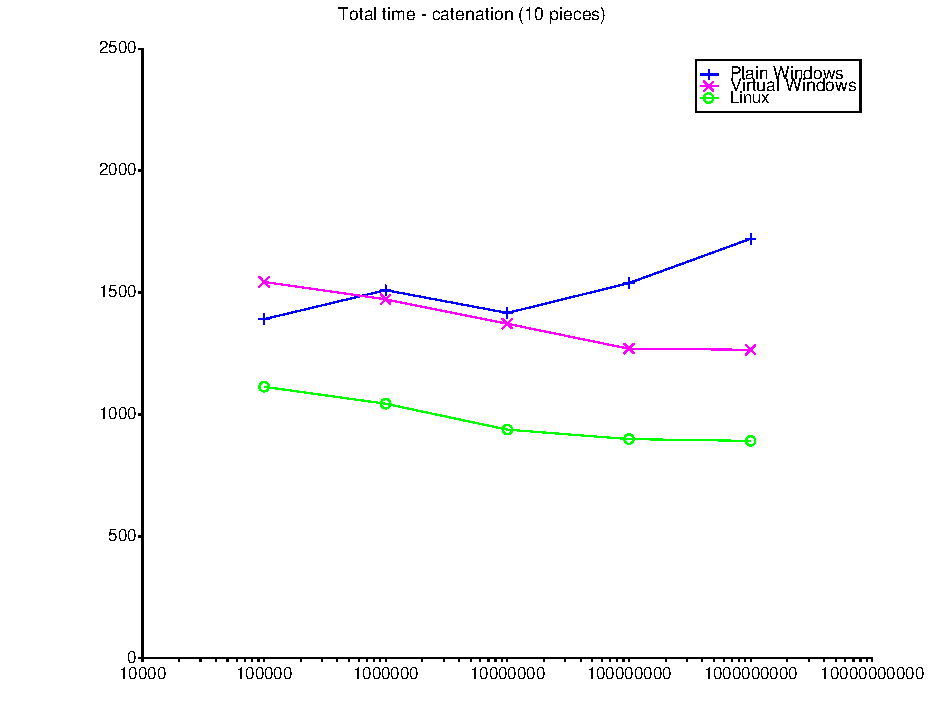
\includegraphics[width=0.9\textwidth]{total_view10.pdf}
\caption{Timings using 10 catenation steps}
\end{figure}

\begin{figure}
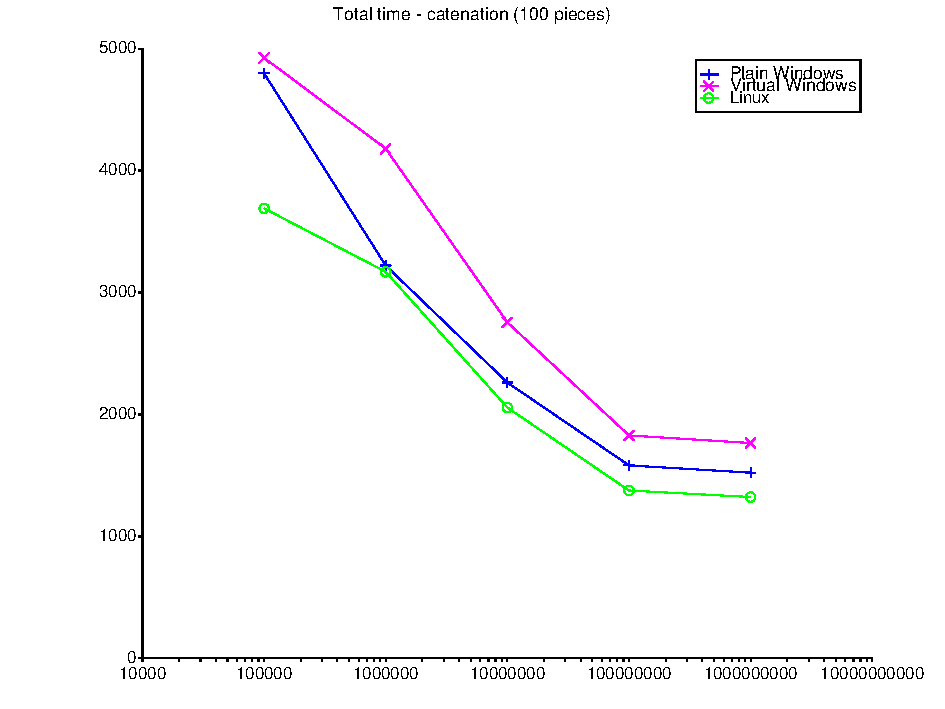
\includegraphics[width=0.9\textwidth]{total_view100.pdf}
\caption{Timings using 100 catenation steps}
\end{figure}

The timings were obtained by repeating a loop a large number of times. In the loop array elements
were accessed at various intervals. The total time is displayed.

Note that the times for the plain arrays are much lower than when using catenation. This has led to a
search for a better performance (see the table).

The first attempt at improvement was to change the \verb+moa_basic_view+ type to a "plain" derived type instead
of a class. The reason: it takes time to construct such objects. But that made no difference in timing.

Thanks to J\'er\'emie van der Plas, a major improvement was achieved by replacing the two lines:
\begin{verbatim}
    shp = view%array(i)%shp
    sz  = shp(1)
\end{verbatim}
\noindent by:
\begin{verbatim}
    sz = view%array(i)%shp(1)
\end{verbatim}

(The Intel oneAPI tool "Inspect" shows in detail where the hotspots are located in the code, up to the
statement level.)

The results are shown in the next two figures. The details of the timings are not entirely consistent, but
roughly it meant a gain of 30\% (at least for some cases, the timings vary a lot).

\begin{figure}
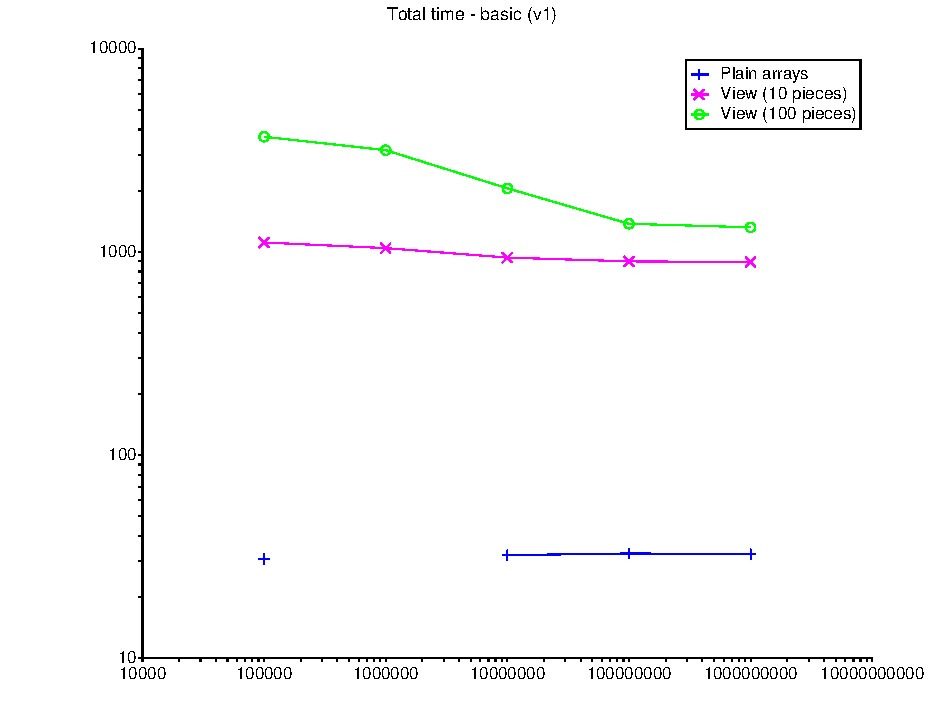
\includegraphics[width=0.9\textwidth]{total_v1.pdf}
\caption{Timings for the different cases (platform: Linux), using the original implementation (version 1)}
\end{figure}

\begin{figure}
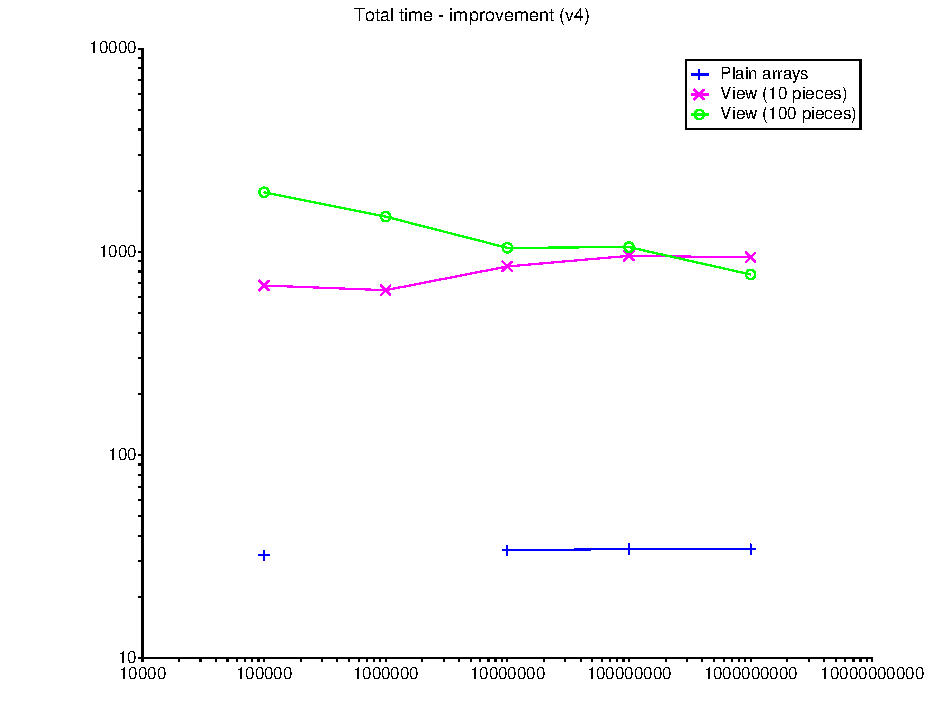
\includegraphics[width=0.9\textwidth]{total_v4.pdf}
\caption{Timings for the different cases (platform: Linux), using the optimisation of version 4.}
\end{figure}

\section{Using compiler flags}
The next improvement was to use the compiler flags \verb+-march=native -mtune=native+ for the gfortran compiler.
The gain is roughly a factor 1.5 to 2 (note the logarithmic scale). A lot more can be done of course with specific
optimisation flags, but that is not realised yet.

\begin{figure}
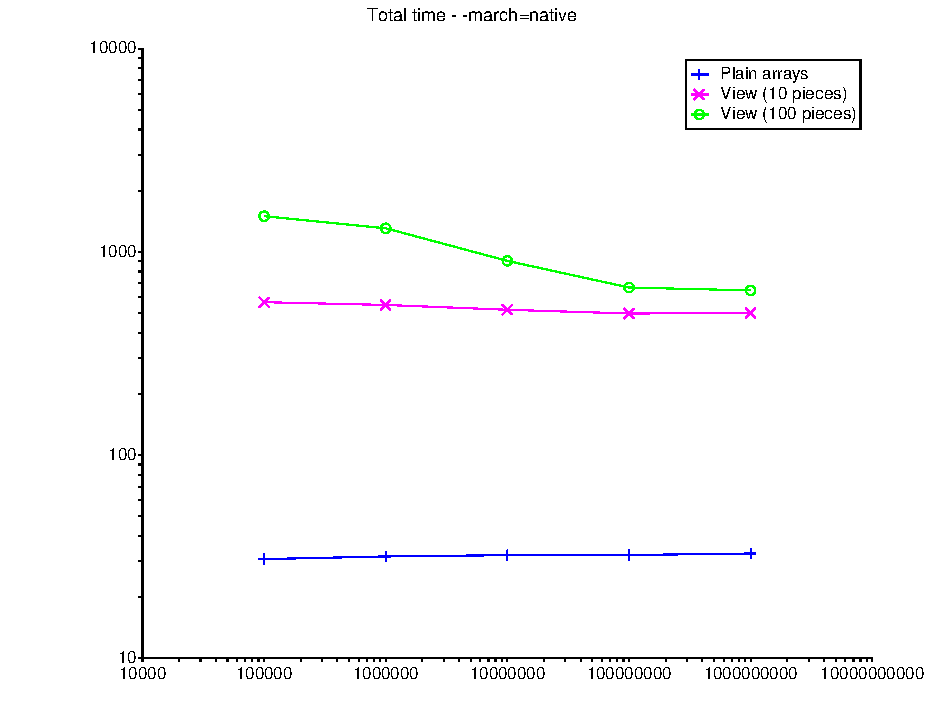
\includegraphics[width=0.9\textwidth]{total_native.pdf}
\caption{Timings for the different cases (platform: Linux), using the "native" compiler flags.}
\end{figure}

\begin{figure}
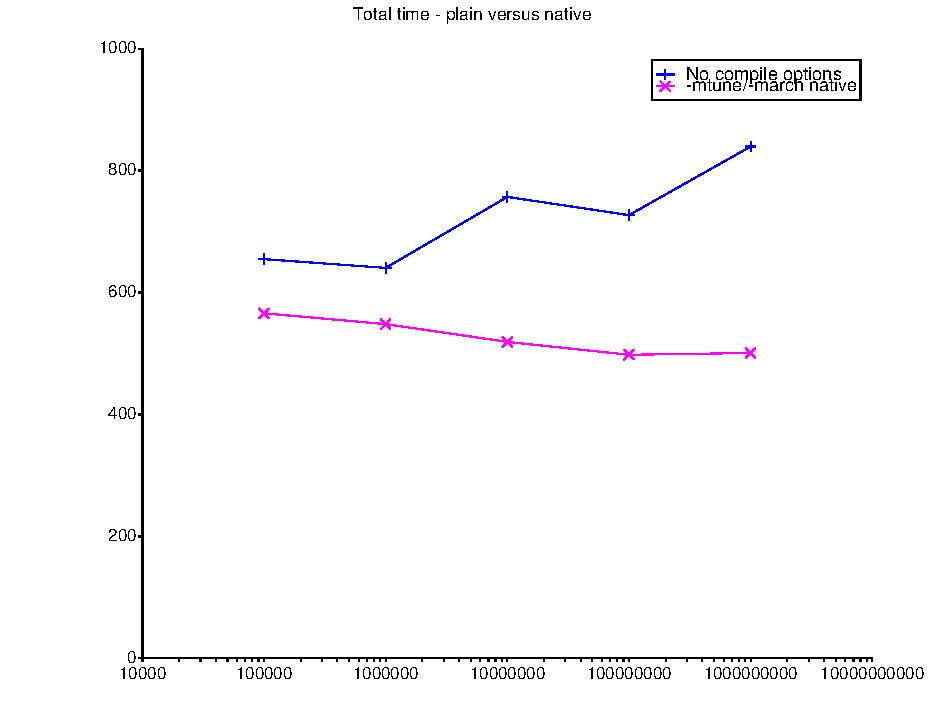
\includegraphics[width=0.9\textwidth]{total_plain_native.pdf}
\caption{Timings for the different cases (platform: Linux), comparison of the "plain" calculation and the
optimised calculation (using the "native" compiler flags.}
\end{figure}

\section{Notes}
Please note that the timings were achieved on computers that were not tuned for this. A lot of background
processes were going on at the time, which makes the timings vary more than is appropriate.

\section{Next steps}
While further optimisation is possible (via analysing the hotspots presented by the Intel oneAPI tool "Inspect"), we
also want to know more about the memory management. Basically: measure the time it takes to extend an array
in plain Fortran and using the MoA catenation technique.

In plain Fortran you can use a loop like:

\begin{verbatim}
    ALLOCATE( array(0) )
    DO i = 1,appends
        array = [array, chunk]
    ENDDO
\end{verbatim}

This relies on the automatic reallocation feature. It constructs a larger array and copies the data in the old array
into the new one. The question is: how expensive is this?

The first results are shown in the figure. This is for plain Fortran only.

\begin{figure}
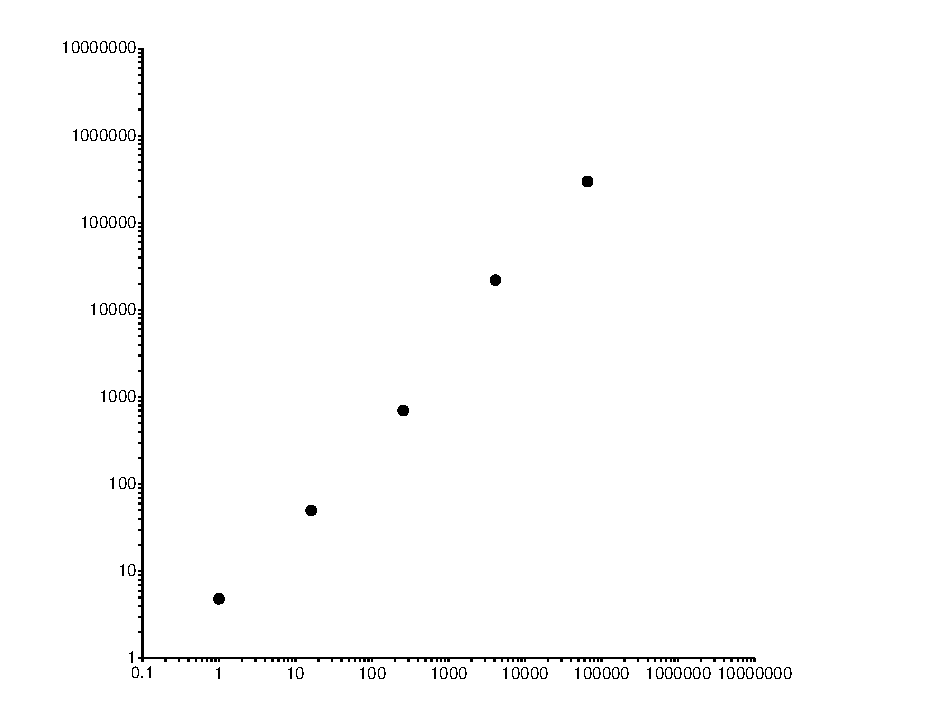
\includegraphics[width=0.9\textwidth]{copy_extend.pdf}
\caption{Timings for copying and extending arrays.}
\end{figure}

The figure shows the time it takes to (in seconds) to extend the array one hundred times by adding another array of
fixed size (the horizontal axis). This was repeated 100,000 times to make sure that sufficient time was consumed.
The data points show an almost linear relationship between the fixed size of the added array and the time.

Now we want to know what happens if you use the MoA catenations.

\end{document}
